% ##################################################################################################################
\chapter{Poznan}
\label{ch:poznan}
\hfill \textbf{Authors:} Michal Maciejewski, Waldemar Walerjanczyk

\editdone{This text has undergone the professional edit. Please no grammatical changes anymore! They are most-probably wrong.}

% ##################################################################################################################
At the time of the initial scenario, Poznan (population of over 550\,000), was the fifth largest city in Poland; together with the neighboring suburban area, it made up an agglomeration inhabited by nearly one million people. The \gls{matsim} scenario development for the Poznan agglomeration began in 2012, and the model has been continuously extended and improved. Currently, it is a 24-hour microscopic model of private transport, with a goal of creating a 24-hour, multi-agent activity-based simulation of the Poznan agglomeration, combining both private and public transport.

The road network model was extracted from \gls{osm} and included all roads and link roads (such as entrances or exits from motorways). The final result was a high-detail road network model consisting of 17\,026 nodes and 40\,129 links. This model was calibrated to determine traffic flow parameters for links (\eg flow capacity, storage capacity, free-flow speed) for each of the 13\,modeled road classes \citep{PiatkowskiMaciejewski2012osmNetwork}.

The travel demand model was derived from the official trip-based 4-stage model used by the Poznan city planning department ; this model dates back to 2000, but has been frequently updated since then. Since the official model was originally designed for morning and afternoon peak hours, it had to be extended to describe travel demand throughout the day, hour after hour. As a result, demand for private transport is represented by 24\,sets of hourly \gls{od} matrices, each set consisting of nine different matrices, one for each of nine travel motivations, namely home $\rightarrow$ work/education/shopping/other, work/education/shopping/other $\rightarrow$ home, and not related to home. This adds up to 216\,\gls{od} matrices \citep{PiatkowskiEtAl2013Poznan24hSimulation, MaciejewskiEtAl2014MikroMakro}.

The official model divided the agglomeration into less than 400\,zones, insufficient for activity locations to be accurately modeled at the microscopic level. To increase accuracy, \gls{osm} land use data was used. Six types of land use---residential, industrial, green, commercial, schools and unclassified---were used to subdivide zones into homogenous subzones. As a result, home activities were located in residential subzones, education activities at schools, shopping in residential or commercial subzones, and so on. Figure~\ref{fig:poznan_home_distribution} illustrates the distribution of \emph{home} locations when land use was taken into account \cite{PiatkowskiMaciejewski2013LandUse}.

%---------------------------------------------------------------------
\createfigure%
{Distribution of home activities based on land use}%
{Distribution of home activities based on land use}%
{\label{fig:poznan_home_distribution}}%
{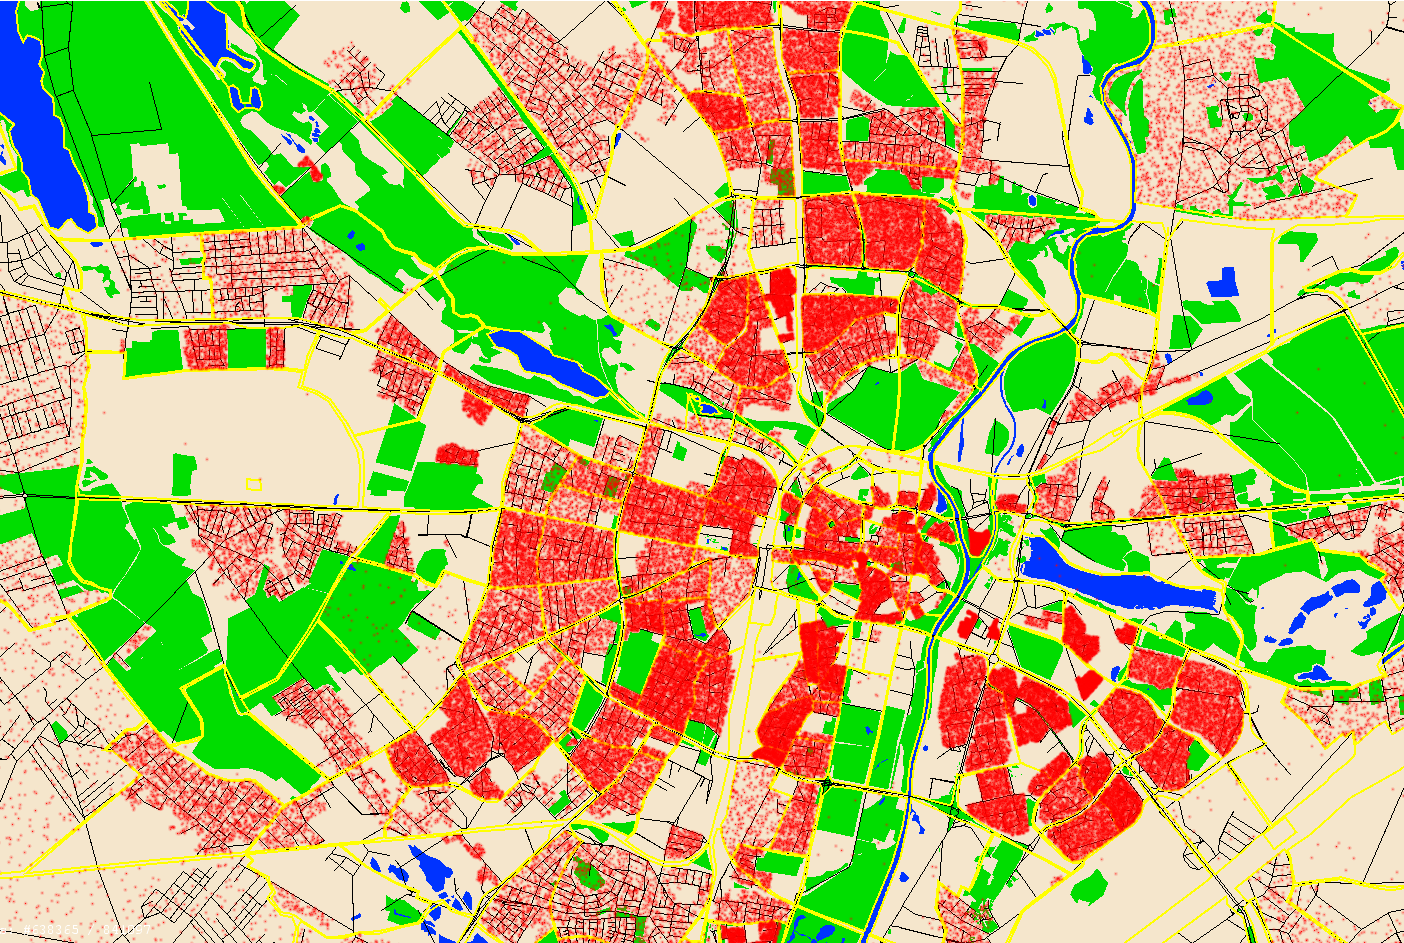
\includegraphics[width=\textwidth, angle=0]{scenarios/figures/poznan_home_distribution}}%
{}%
%---------------------------------------------------------------------

Having calculated the \gls{od} matrices for private transport and subdivided the area into homogenous subzones, the next step was to generate agents population. In the first attempt, it was assumed that each agent performed only one trip, so the number of agents equaled the demand represented by the \gls{od} matrices, which was almost 840\,000. Departure times were randomly distributed (uniform distribution) over each hour, and therefore, the only decision made by each agent during the replanning phase concerned the route choice for the preselected pair of locations. The whole simulation consisted of 120\,iterations, yet it usually takes about 60\,iterations to achieve a relaxed state. Figure~\ref{fig:poznan_traffic_simulation} showed the state of traffic at 7\,am.

%---------------------------------------------------------------------
\createfigure%
{Road traffic in the Poznan agglomeration at 7\,am}%
{Road traffic in the Poznan agglomeration at 7\,am}%
{\label{fig:poznan_traffic_simulation}}%
{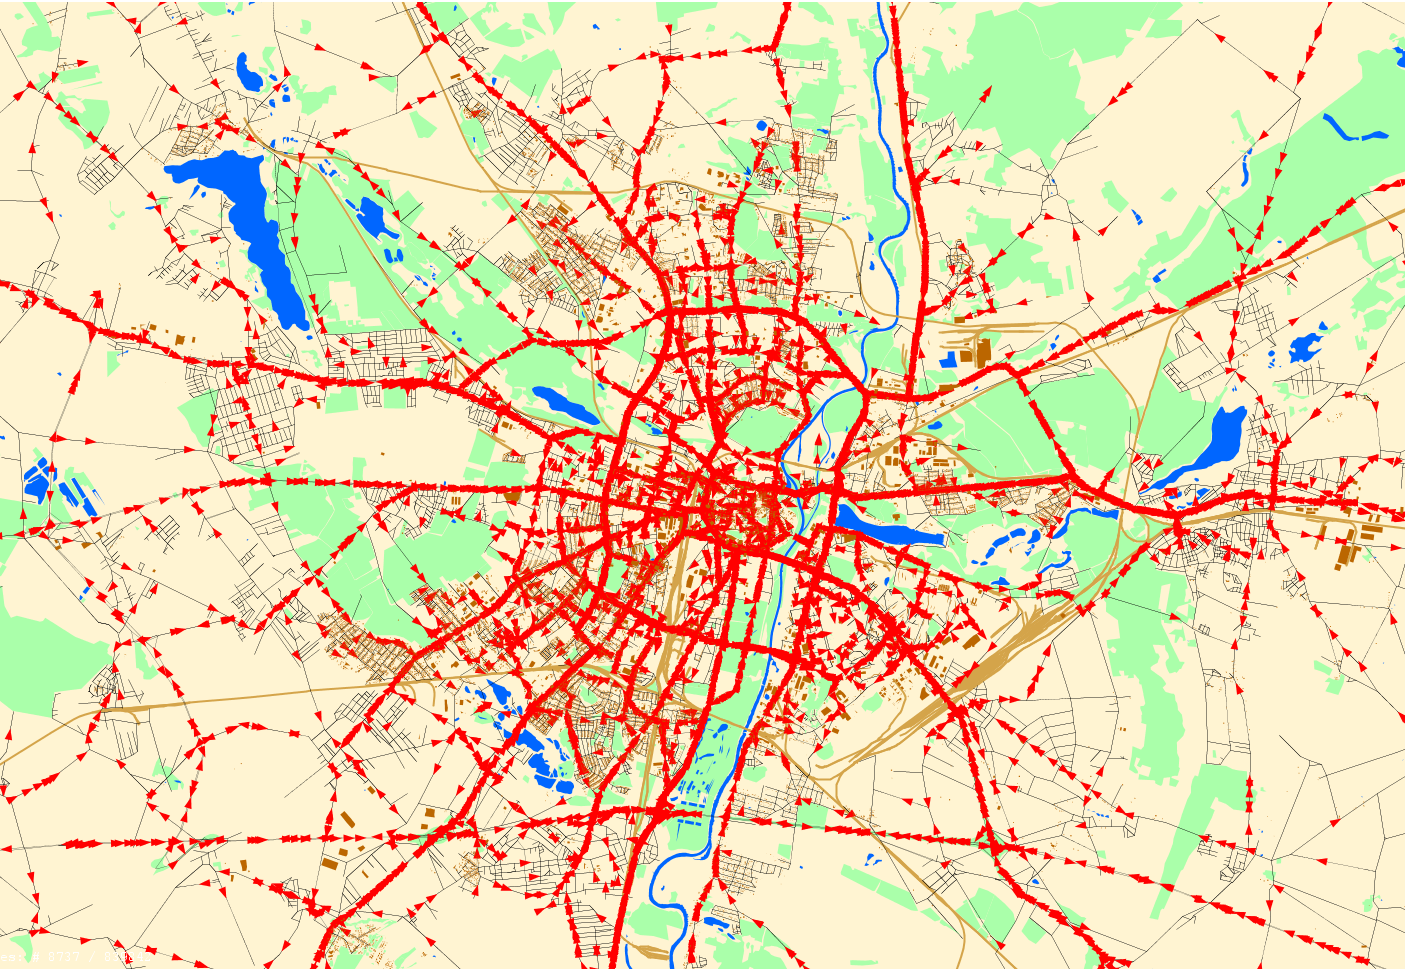
\includegraphics[width=\textwidth, angle=0]{scenarios/figures/poznan_traffic_simulation}}%
{}%
%---------------------------------------------------------------------

Currently, the model is being updated according to a comprehensive travel study carried out in 2014. At the same time, the public transport system is being added, allowing for simulation of both private and public transport. The Poznan model has been used for simulation of real-time electric taxi dispatching, done through the \gls{dvrp} \gls{contribution} (see Chapter~\ref{ch:dts}).

% ##################################################################################################################
